\chapter{Requirements}

In the previous chapter, we have described some tools that provide debugging mechanisms that would also be useful for cross-device testing and debugging. However, most of those mechanisms need to be extended to fulfill the needs of a cross-device testing and debugging tool. In the following sections, we will describe the key requirements for such a tool, i.e. XDTools.

\section{Emulation of Multiple Devices}

Device emulation is already very popular for testing responsive websites. The number of physical devices that a developer has access too is typically rather limited, thus testing on emulated devices helps cover a wider range of devices. In its simplest form, device emulation is just resizing a browser window so it looks and feels like a device with a different resolution. However, manually resizing a browser window such that it has the exact resolution of a real device is difficult. Furthermore, just changing the screen size does not realistically emulate a real device: Mobile devices typically use touch interactions, often have poor network connectivity and have access to a wide range of sensors. Those limitations have led to the emergence of more sophisticated tools for device emulation. Advanced device emulation tools such as the Device Mode in Chrome DevTools emulate different screen sizes, touch capabilities, network conditions, as well as location and acceleration sensors. They also typically provide a list containing some existing devices. In addition, the developer can create custom devices. However, all such tools have one limitation in common: They can emulate only one device per browser tab or window and even if multiple browser windows are used, those browser windows share the same local resources such as local and session storage. This limits the usefulness of such tools for cross-device application testing. Cross-device applications typically run on multiple independent devices simultaneously and thus should not share any local resources. In practice, developers employ a number of different mechanisms to prevent the sharing of local resources: First, multiple different browser profiles can be used. Second, the incognito mode provided by most browsers can be used to prevent sharing of local resources. Lastly, multiple independent browsers can be used. However, those solutions all have some limitations: Using multiple independent browsers obviously limits the number of devices that can be emulated to a rather small number and requires the installation of all those browsers. Also, all those solutions require the developer to open multiple windows simultaneously and arrange them on the screen. This is tedious and frequent switching between browser windows is required. Furthermore, tasks like creating multiple browser profiles are time-consuming and might not be what the developer wants. Finally, not all browsers support multiple browser profiles, limiting the number of browsers on which an application can be tested. But not only the process of emulating multiple devices itself is tedious: If the developer actually wants to use browser debugging tools, those tools have to be opened for each window separately which requires additional screen space. The screen space of the developer's machine can also be a limiting factor: If the screen has a full HD screen but the developer wants to emulate a full HD device as well as some mobile devices simultaneously, those devices cannot be ordered such that all devices are visible at the same time. The developer would need to put one window in full screen and switch browser windows when they want to access the other devices. Constantly switching between devices can be tedious and the consequences of interactions performed on one device cannot be observed in real-time on other devices because switching between windows requires some time. Also, emulating resolutions larger than Full HD, e.g. a 4k TV, is even more difficult.

Those limitations all contribute significantly to the difficulty of cross-device application testing. Using these limitations, we gathered a number of requirements for device emulation in XDTools:
\begin{itemize}
	\item It should be possible to \emph{emulate multiple devices} in one browser window.
	\item The emulated devices should \emph{not share any local resources}. The solution for preventing the sharing of local resources should be \emph{scalable and robust}.
	\item The screen size should not be a major limiting factor concerning the number of devices that can be emulated simultaneously. This can be realized by \emph{scaling devices} down without changing their resolution.
	\item The developer should have access to a list containing some \emph{existing devices}.
	\item The developer should be able to \emph{dynamically change the resolution} of emulated devices.
	\item The developer should be able to add and save \emph{custom devices}.
\end{itemize}

Scaling devices down while keeping the resolution and resizing devices are two different concepts. The difference between the two is illustrated in Figure~\ref{fig:difference_resizing_scaling}.

\begin{figure}[H]
  \centering
    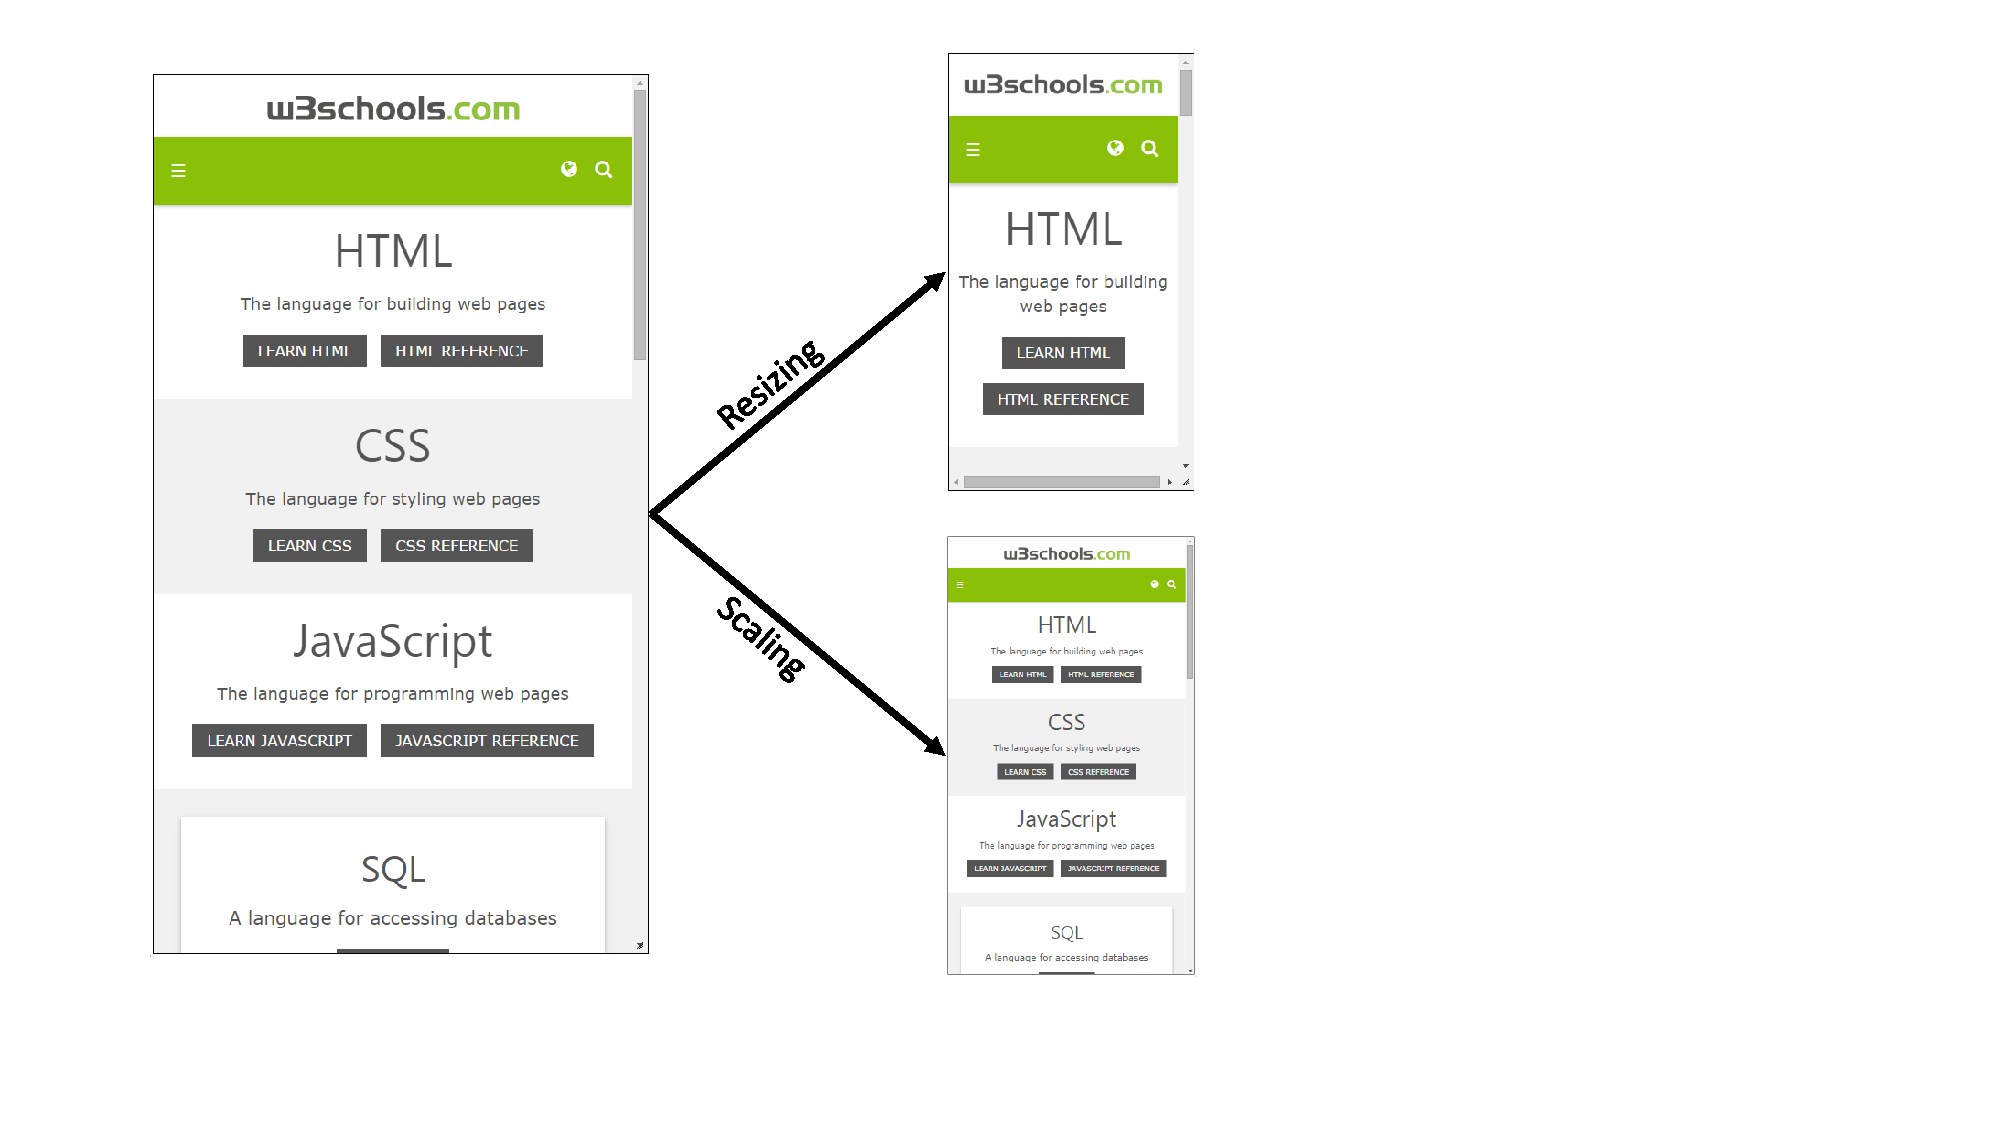
\includegraphics[width=1.0\textwidth]{images/difference_scaling_resizing.pdf}
	\caption[Difference between resizing and scaling a device]{Difference between resizing and scaling a device}
	\label{fig:difference_resizing_scaling}
\end{figure}

\section{Easy Integration of Real and Emulated Devices}

Emulating devices is a versatile tool for testing applications on many different devices. However, it does not completely eliminate the need for testing on real devices: Device emulation is always limited to certain aspects that are being emulated, e.g. screen size, resolution, touch interactions and location. However, not every little detail of a real device can be emulated accurately. The following list provides an overview of some of the other limitations regarding testing on emulated devices:
\begin{itemize}
	\item Touch interactions: Even though modern device emulators can also emulate touch interactions, performing a gesture with the mouse will never feel the same as the actual touch interaction. An interaction that works great with the mouse might feel awkward when performed on a real device and vice-versa. Also, multi-touch interactions such as pinching are difficult to emulate in a realistic way on an emulated device without real touch support.
	\item Interrupts: While using an application on a real device, the user might be interrupted by many different things, e.g. the arrival of a text message. Those interrupts cannot be simulated in a realistic way on an emulated device.
	\item Performance: A desktop PC typically has much more computing power than a mobile device. If an application performs poorly on mobile devices, this might not even be noticed if the developer only tests on emulated devices.
	\item Display: The display quality and thus also the look of an application varies greatly depending on the device. Only emulating devices on a desktop PC cannot account for those differences in display quality. 
	\item Sensors: Modern devices have a large number of different sensors that cannot all be emulated realistically. One particular problem is the orientation of the device: A user might switch between landscape mode and portrait mode on purpose or accidentally at multiple points. Although the orientation of emulated devices can also be switched, this does not accurately simulate the behavior of a real user.
\end{itemize}
Although this list gives a good overview of the limitations of testing on emulated devices only, it is by far not complete and what happens on a real device cannot always be foreseen by testing on emulated devices. Thus, testing on real devices is crucial for the successful development of a cross-device application. 

The importance of testing on real devices leads to a new requirement for XDTools: It should easily be possible to \emph{connect real devices} to XDTools. 

\section{Easy Switching of Device Configurations}

Cross-device applications are typically used by different groups of users and thus also different devices. Even the same user may sometimes use their mobile phone and laptop simultaneously and at other times only their mobile phone or tablet. Thus, the number of devices that are used simultaneously cross-device application and those devices' characteristics may vary greatly. Depending on the devices connected to a cross-device application, the UI distribution and the behavior of the application might be different. A cross-device application needs to be able to support all different device scenarios. Some cross-device applications are targeted to specific scenarios, e.g. a presentation room with multiple big screens that are always present, as well as some mobile devices that are only in the room when their owner is attending a presentation. In such a scenario, the developer would probably want to have access to the two static devices whenever they are testing the application and dynamically add some mobile devices. However, in other scenarios there might be no static devices at all, e.g. a public place where all visitors can connect their devices to an application related to the place. Due to the large number of different device scenarios that could be used with a cross-device application, it is a key requirement for XDTools that the developer can quickly \emph{create multiple different device scenarios} and \emph{easily switch} between those device configurations. 

\section{Integration with Debugging Tools}

Many of the features integrated into the debugging tools of browsers are also immensely useful for debugging cross-device applications, and some might even help more when debugging cross-device applications than when debugging traditional web applications. However, those tools are limited to debugging one device at a time. We have established before that XDTools should allow emulation of multiple devices in the same browser window. While this already simplifies the debugging of multiple devices somewhat, it also introduces some new difficulties. The messages that are logged from the emulated devices are all shown in the browser debugger tools of the same window. This aggregation of logging messages is useful for seeing the messages from all devices at one glance, but identifying the device that a message came from is more difficult. The same limitation applies to JavaScript errors that are shown in the console but cannot easily be related to a device. Also, trying out things in the console by sending commands to devices becomes more difficult. Google Chrome allows the developer to switch between different frames in the console and thus address different frames with commands, but it is not always obvious which frame corresponds to which device. Also, the developer might want to try out the same thing on multiple devices and would have to switch between multiple frames to address all of them. Further limitations of the browser-included debugging tools include that navigating to the HTML of an emulated device can be rather tedious, that CSS can only be applied to one device at a time and that function breakpoints can only be added on one device at a time. Especially the last limitation can make cross-device application testing difficult because different devices have different responsibilities and not all devices might use all JavaScript functions. Consequently, adding a breakpoint inside a function on one device might not help with debugging the function at all, if the function is not called on that device. The existence of real devices complicates things even more. By connecting the device to the desktop PC via cable, the developer gets access to remote debugging, but debugging multiple devices at the same time gets even more complicated. The remote debugging of each device is opened in a new window, thus the developer once again has to navigate between multiple windows, something that we wanted to avoid by emulating multiple devices in one browser window. Also, getting an overview of the logging messages from all devices and sending commands to multiple devices becomes even more difficult. However, integrating existing debugging tools into XDTools is clearly desirable: Most of those tools have been around for quite some time. Thus, they are already well tested and have gone through a series of improvements. Also, almost all web developers have already used those tools for extensive testing and are already familiar with them. However, XDTools needs to extend those tools to support debugging on multiple devices simultaneously. Using all this information, we derived the following requirements for XDTools:
\begin{itemize}
	\item Logging messages from all devices should be aggregated in one place and the device the messages originated from should be easy to identify.
	\item JavaScript errors from all devices should be aggregated and easily identifiable.
	\item Sending JavaScript commands to multiple devices at a time should be possible and easy to achieve. 
	\item It should be easy to inspect the HTML of specific devices.
	\item It should be possible to add CSS to multiple devices at the same time (see Figure~\ref{fig:css_aggregation}).
	\item The developer should be able to add breakpoints to multiple devices simultaneously.
	\item If technically feasible, all of the above requirements should be applied to both real and emulated devices.
\end{itemize}

\begin{figure}[H]
  \centering
    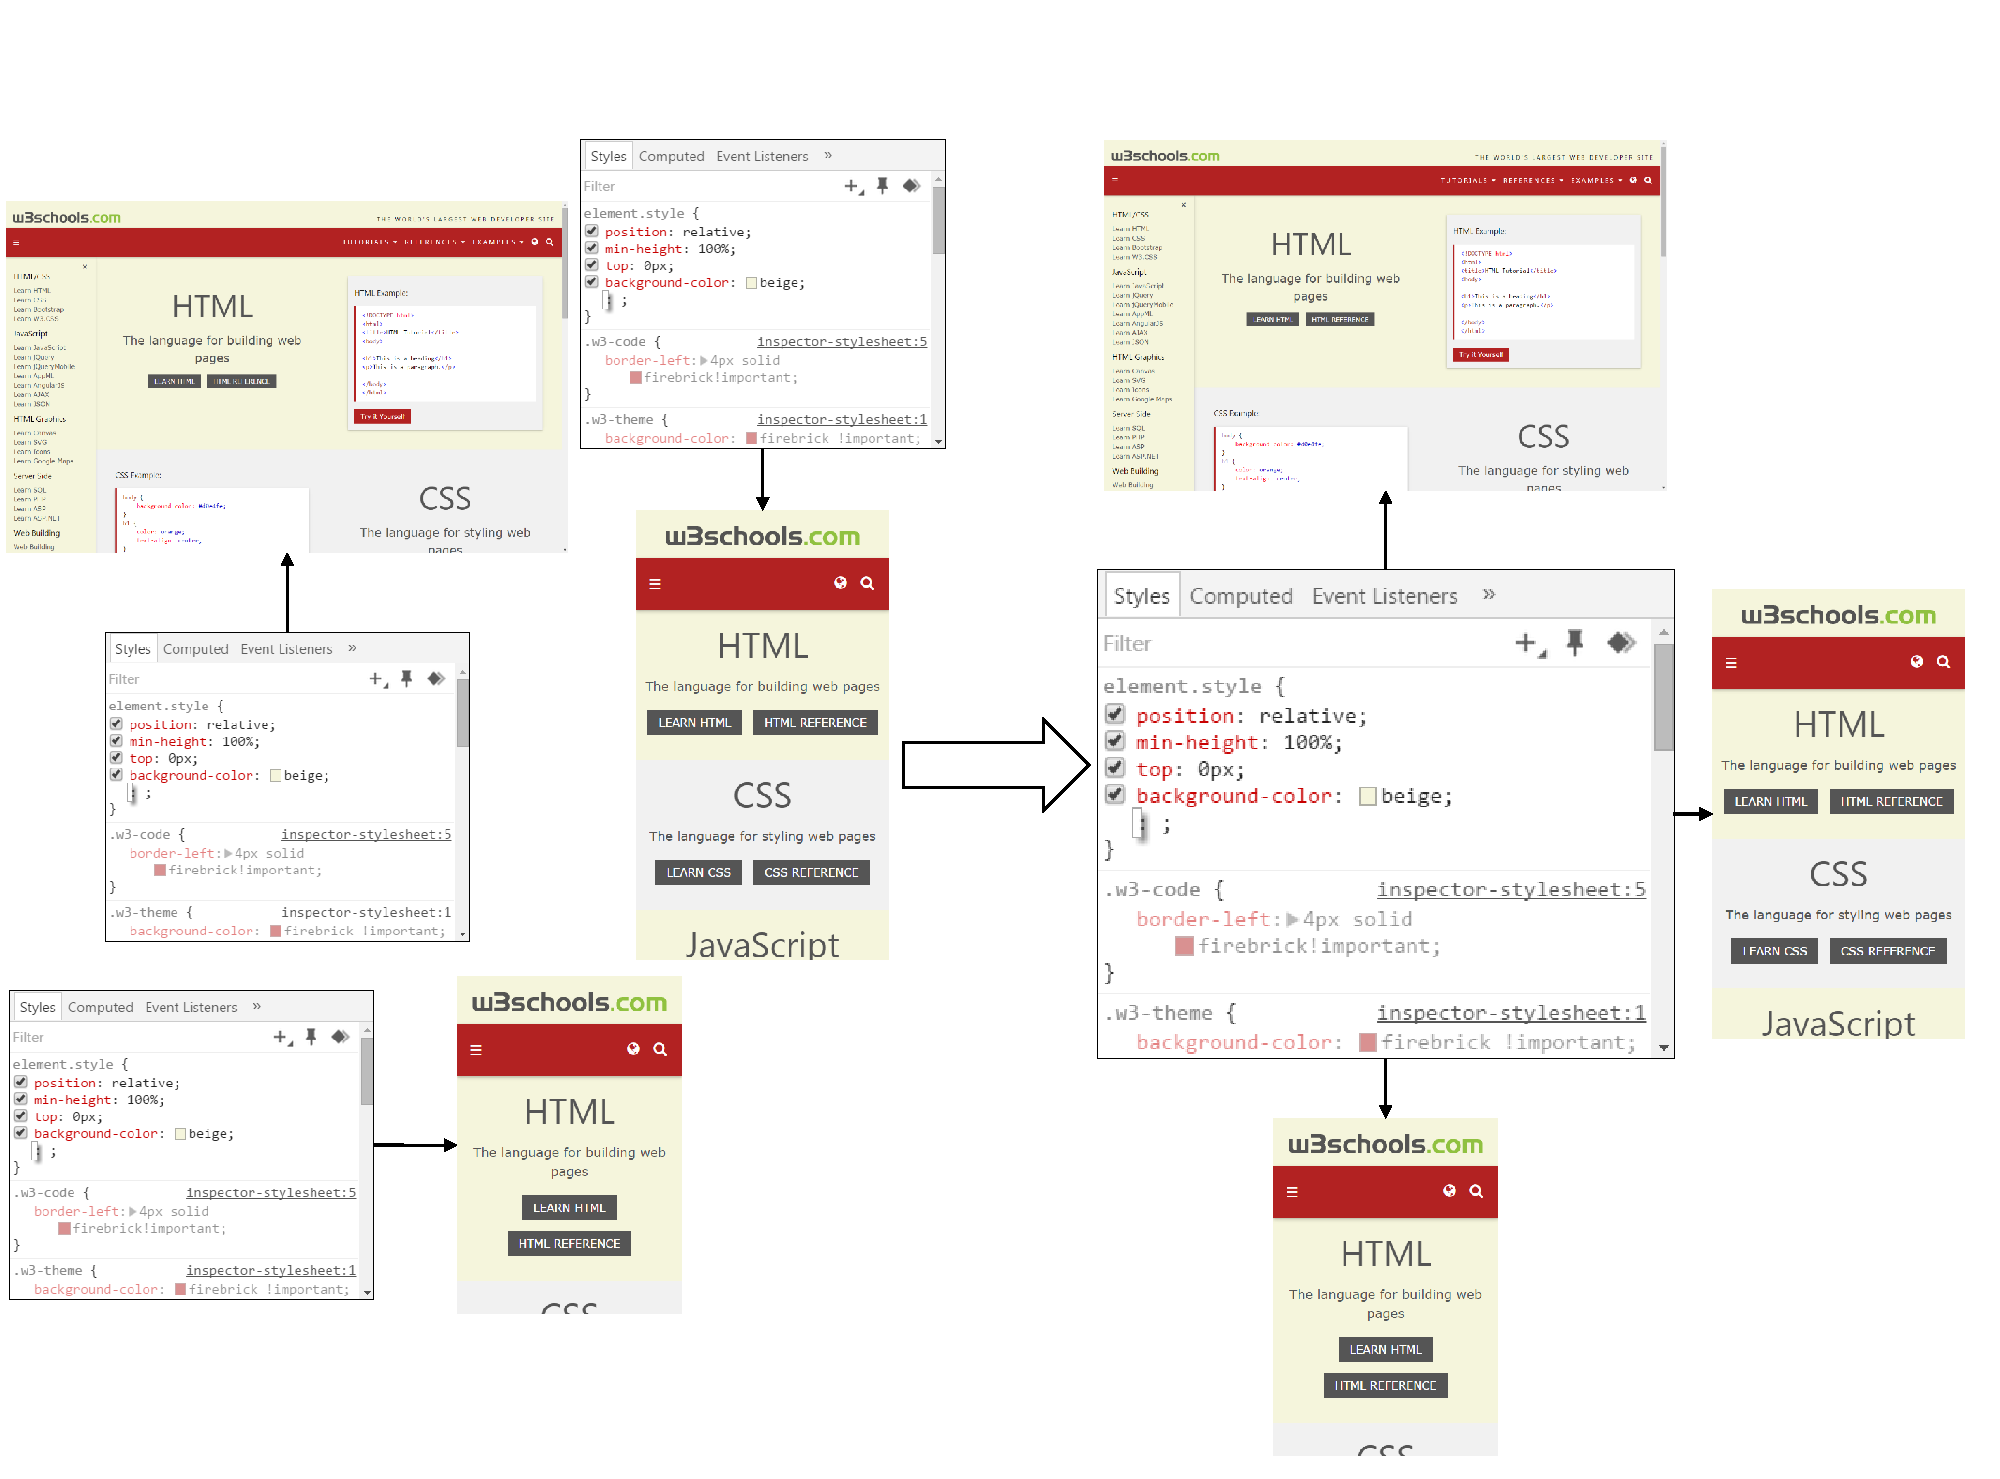
\includegraphics[width=1.0\textwidth]{images/css_aggregation_4.pdf}
	\caption[CSS editor aggregation]{CSS editor aggregation}
	\label{fig:css_aggregation}
\end{figure}

\section{Automatic Connection Management}

In order to use a cross-device application with multiple devices simultaneously, those devices need to be paired with each other. The mechanisms for pairing devices differ between the various cross-device application frameworks: With some frameworks, all devices that open the cross-device application are paired implicitly. In other frameworks, for example XD-MVC, devices can be paired by copying the URL from one device to the other devices. Other frameworks have more complicated mechanisms for connecting devices. In Connichiwa, one device runs a local web server and uses Bluetooth to detect nearby devices. The device then sends the IP of the web server over Bluetooth, enabling the other devices to access the received IP in a web browser. All of those mechanisms have one thing in common: Devices are connected by opening a specific URL in the browser. However, other ways of connecting devices are also feasible: Some frameworks provide a function that can be called from one device to connect the device to another device. Also, many of the papers describing cross-device application development frameworks do not describe how devices are connected. Finally, cross-device applications can also be implemented independently of any framework and might use completely different mechanisms for connecting devices. Thus, it is impossible to derive all mechanisms that could possibly be used for connecting devices in a cross-device application.

However, if the developer wants to debug a cross-device application, reconnecting the devices every time a new device configuration is loaded or possibly even when devices are refreshed is tedious and time-consuming. Thus, it is desirable to have some easy way of connecting devices. From this, we derive the next requirement for XDTools: It should be possible to \emph{automatically and manually connect devices} to each other. If possible, the provided connection mechanism should work \emph{independent} of the connection mechanism used in the cross-device application under test.

\section{Coordinated Record and Replay}

Record and replay has been used previously for recording and replaying user interactions in traditional web applications and especially AJAX web applications. The non-deterministic and asynchronous nature of web applications contributes much to the value of record and replay in web applications. When a bug is encountered in a web application, it is often difficult to determine the exact steps for reproducing the bug. Reproducing bugs becomes even more difficult in cross-device scenarios where multiple devices are involved and the interactions performed on one device have implications on other devices. Also, cross-device applications are often used by multiple users at the same time and it is difficult for one developer to simulate multiple users interacting with their devices simultaneously. Thus, we believe that record and replay can benefit cross-device application developers even more than developers of traditional web applications. However, precise mechanisms for timing the replay are needed if we want to simulate multiple users simultaneously. Also, simply replaying interactions is not enough: If something goes wrong in the application, we need some way of pausing the replay and inspecting the state of the devices. XDTools should implement a record and replay mechanism that fulfills the following requirements:
\begin{itemize}
	\item All \emph{interactions} with the device should be \emph{recorded}. 
	\item It should be possible to \emph{replay a sequence of interactions on another device} than the device that recorded the sequence.
	\item It should be possible to \emph{pause the replay} of the interaction sequence.
	\item \emph{Accurate timing} of replays should be possible.
	\item The developer should be able to \emph{store event sequences} for later use, e.g. for testing them again in future iterations of the application under test.
\end{itemize}